\subsection{Evaluation Lösungsprinzipien}\label{mk}

Aus der vorhergehenden Technologierecherche (siehe Anhang \ref{techrecherche}) wird pro Teilbereich ein morphologischer Kasten erstellt. Dieser wird befüllt mit den Teilfunktionen und den recherchierten Technologien. Damit werden die Lösungsprinzipien evaluiert und verschiedene Varianten werden ausarbeitet. Nachfolgend sind alle morphologischen Kästen aufgezeigt.

Die Lösungsvarianten wurden gewählt anhand der Muss-Kriterien, die erreicht werden sollen: Simpel, nicht zu teuer, nicht die 30cmx30cmx80cm ausnutzen, Robustheit. Zusätzlich wurde in Betracht gezogen, wie stimmig die einzelnen Technologien miteinander sind.

\subsubsection{Mechanik Morphologischer Kasten}

Auf Basis der Technologierecherche (siehe Anhang \ref{techrecherche}) wurden verschiedene Lösungsansätze für die einzelnen Teilfunktionen ausgewählt und in den morphologischen Kasten aufgenommen.  Diese Lösungsansätze wurden nach folgenden Kriterien erstellt.

\begin{itemize}
    \item Variante Gelb: Effizient
    \item Variante Rot: Präzise
    \item Variante Grün: Robust
\end{itemize}

\begin{table}[H]
\centering
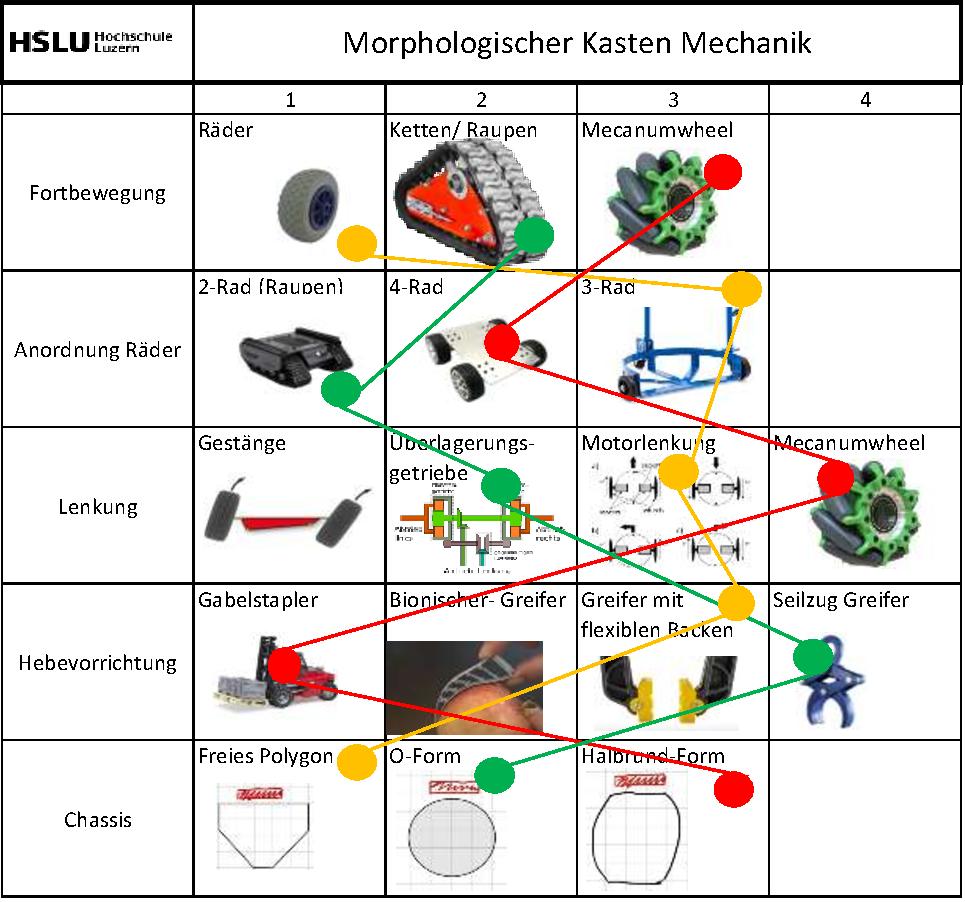
\includegraphics[width=0.7\textwidth]{assets/MK_Maschinentechnik.pdf}
\caption{Morphologischer Kasten: Mechanik}
\label{table:mk-mechanik}
\end{table}


\subsubsection{Steuerung Morphologischer Kasten}

Aus der Technologierecherche (siehe Anhang \ref{techrecherche}) entstand folgender morphologischer Kasten mit drei Varianten für die Teilfunktionen, die die Elektronik und die Steuerung im Roboter bilden. Diese wurden jeweils nach folgenden Kriterien zusammengestellt.

\begin{itemize}
    \item Variante Gelb: Simpel
    \item Variante Rot: Austauschbar
    \item Variante Grün: Präzise
\end{itemize}


\begin{table}[H]
\centering
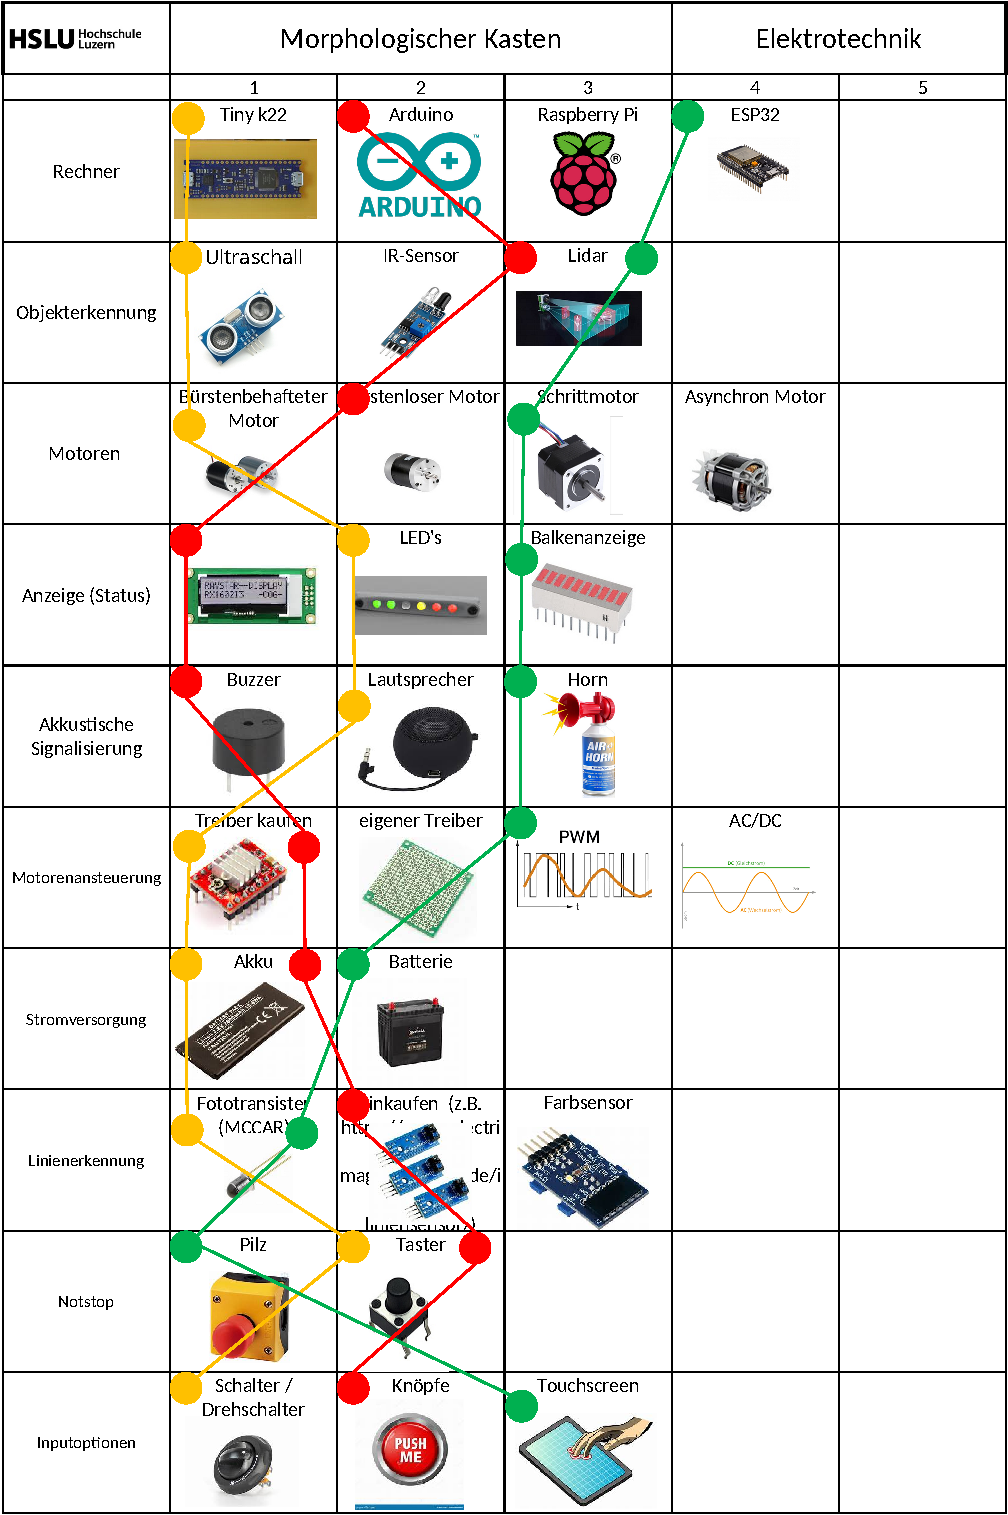
\includegraphics[width=\textwidth -5mm]{assets/MK_Elektrotechnik.pdf}
\caption{Morphologischer Kasten: Steuerung}
\label{table:mk-elektrotechnik}
\end{table}

In allen drei Varianten ist konsequent ein Mikrocontroller vorgesehen. Einige Komponenten, wie etwa Buzzer und Lautsprecher oder Drehschalter und Tasten, sind grösstenteils austauschbar. Spezifische Schaltungselemente wie Strombegrenzer und Spannungsregler wurden hingegen nicht im morphologischen Kasten berücksichtigt, da solche Entscheidungen erst während des Layoutprozesses getroffen werden.


\subsubsection{Navigation Morphologischer Kasten}

Aus der Technologierecherche (siehe Anhang \ref{techrecherche}) wurde folgender morphologischer Kasten mit drei Varianten für die Teilfunktionen, die die Navigation bilden, erstellt.  Diese Kriterien wurden jeweils aufgrund folgender Kriterien erstellt.

\begin{itemize}
    \item Variante Gelb: Flexibel
    \item Variante Rot: Sicher
    \item Variante Grün: Leichtgewichtig
\end{itemize}

\begin{table}[H]
\centering
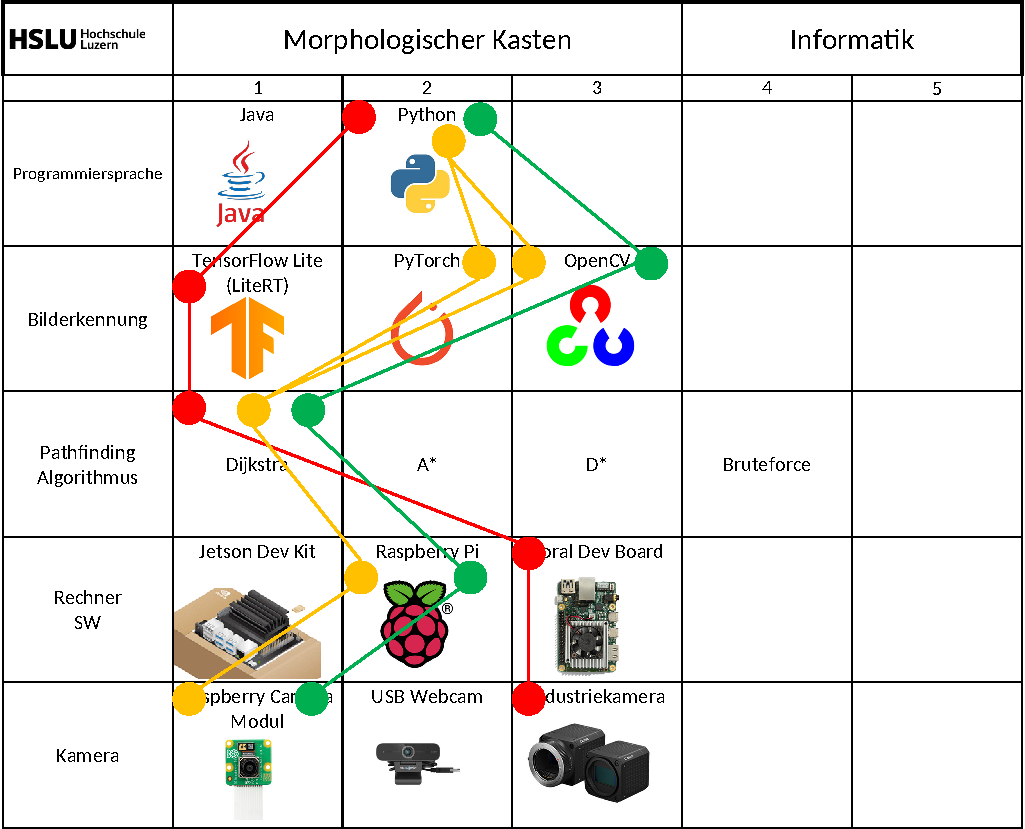
\includegraphics[width=\textwidth]{assets/MK_Informatik.pdf}
\caption{Morphologischer Kasten: Navigation}
\label{table:mk-informatik}
\end{table}


Bei den drei Varianten fällt auf, dass alle Python und den Wegfindealgorithmus Dijkstra verwenden. Python wurde immer gewählt, da Bilderkennung und Machine Learning sehr gut mit Python harmonisieren. Viele Libraries, inklusive dieser, die hier ersichtlich sind, sind kompatibel mit Python. Dijkstra wurde immer gewählt, weil dieser Algorithmus simpel und robust ist und die Geschwindigkeit vernachlässigbar ist. Da es im Graphen nur 8 Knoten gib, wird die Berechnung bei jedem Algorithmus schnell sein.

\subsubsection{Simulator Morphologischer Kasten}\label{mk-simulator}


Aus der Technologierecherche\ref{techrecherche} wurde folgender Morphologischer Kasten für die Teilfunktonen des Simulators erstellt. Es gibt drei Varianten, die in Frage kommen. Diese wurden jeweils nach folgenden Kriterien zusammengestellt.

\begin{itemize}
    \item Variante Gelb: Schnell
    \item Variante Rot: Leichtgewichtig
    \item Variante Grün: Wiederverwendbar
\end{itemize}


\begin{table}[H]
\centering
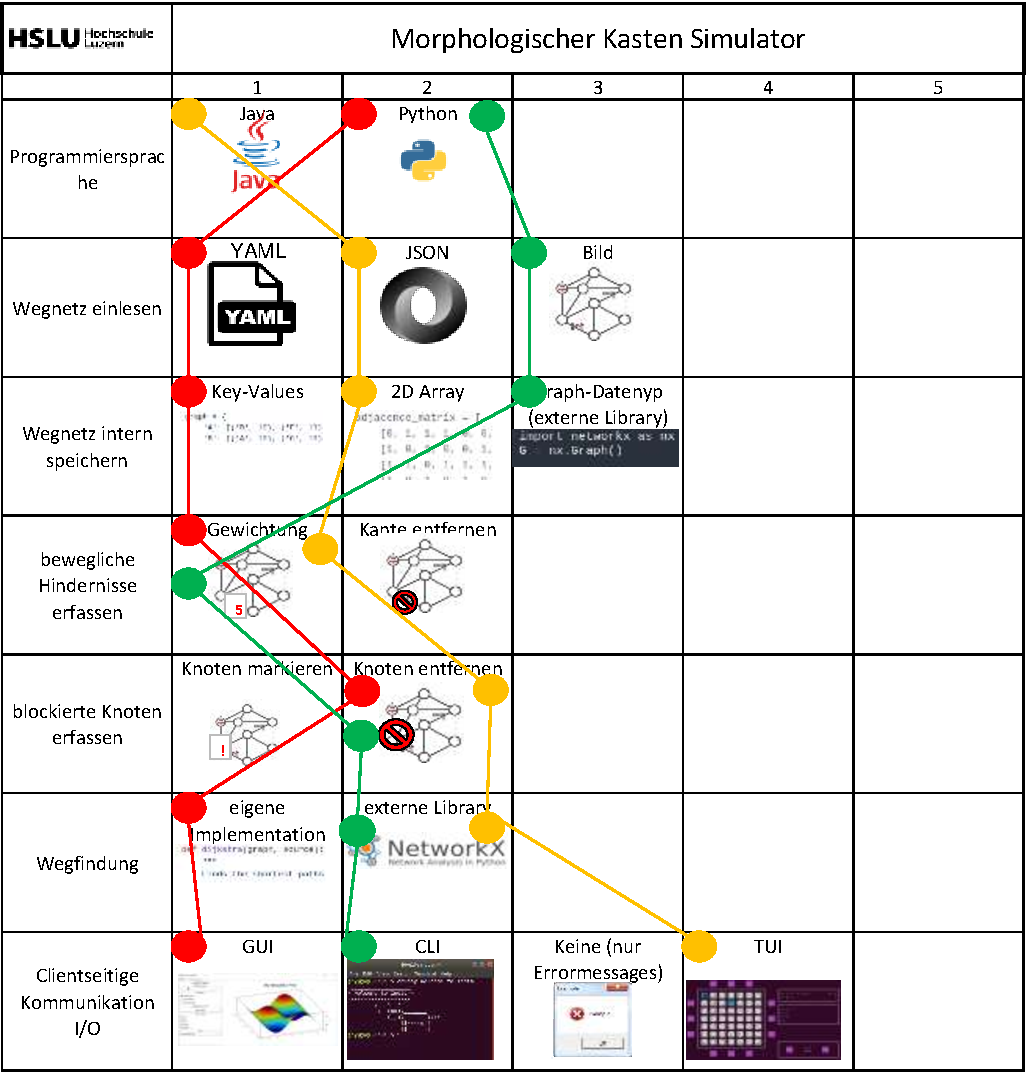
\includegraphics[width=\textwidth]{assets/MK_Simulator.pdf}
\caption{Morphologischer Kasten: Simulator}
\label{table:mk-simulator}
\end{table}



Beim Erfassen von beweglichen Hindernissen wird in jeder Lösungsvariante die Kante nicht entfernt, sondern neu gewichtet. Es ist nicht garantiert, dass es immer einen Weg ohne beweglichem Hinderniss gibt. Diese Strecken zu entfernen, wäre zu risikobehaftet.

Ebenfalls wird ein Knoten immer entfernt falls ein Pylon darauf steht. Er wird nicht markiert, da es würde keinen Vorteil bringen, den Knoten weiterhin zu speichern.


\newpage
\subsection{Auswahl Lösungskombinationen}\label{nutzwertanalyse}

Zur Auswahl der passendsten Lösungskombination wird pro Teilbereich eine Nutzwertanalyse durchgeführt. Die Kriterien und deren Gewichtung sind individuell pro Teilbereich, damit sie ideal passen. Die Variante mit der höchsten Punktezahl ist die Variante, die am besten passt.

\subsubsection{Mechanik Nutzwertanalyse}

Für die  drei Lösungskombinationen aus dem morphologischen Kasten wird eine Nutzwertanalyse gemacht.    

\begin{itemize}
    \item Variante A - Gelb: Zwei von drei Rädern werden direkt durch einen Motor angetrieben. Das dritte Rad ist frei drehend und dient als Stützrad. Das Hindernis wird mit einem Greifer angehoben der zwei flexible Backen hat, die sich optimal an das Hindernis anpassen. Da Variante A nur drei Räder hat, hat das Chassis die Form eines freien Polygons. Diese Variante zeichnet sich durch ihre effiziente Bauweise aus. 
    \item Variante B - Rot: Die vier Mecanum Räder sind auf der halbrunden Grundplatte angeordnet. Jedes Rad wird mit einem seperaten Motor angetrieben.  Das Hindernis wird mit einer Gabel wie bei einem Gabelstapler angehoben. Diese Variante stellt eine präzise Verschiebung des Hindernisses sicher, ist jedoch in in der umsetzung Aufwändiger als die Variante A. 
    \item Variante C - Grün: Der Antrieb erfolgt mit einem Motor und wird mit mithilfe eines Überlagerungsgetriebes auf die einzelnen Raupen übertragen.  Das Hindernis wird mit einem selbst-klemmenden Seilzuggreifer angehoben. Das Fahrzeug wird auf einem runden Chassis aufgebaut. Aufgrund des Raupenantrieb ist die Variante C die Robusteste der drei Varianten. 
\end{itemize}

\begin{table}[H]
\centering
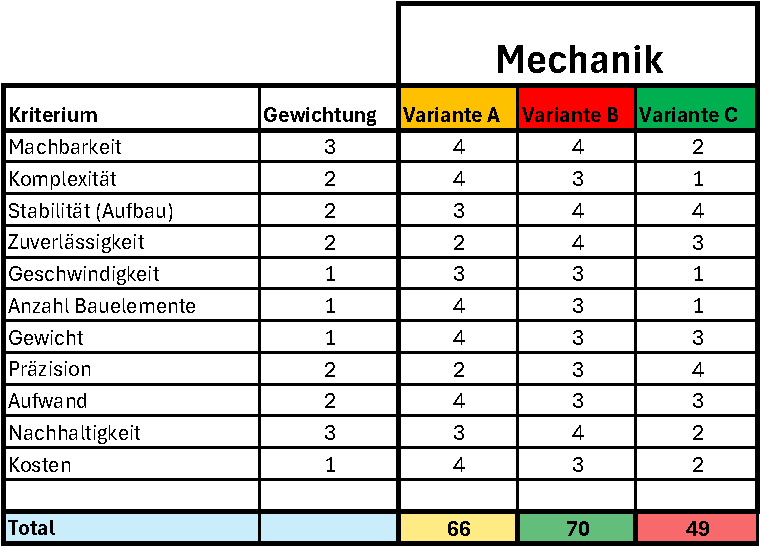
\includegraphics[width=0.75\textwidth]{assets/Nutzwertanalyse-M.pdf}
\caption{Nutzwertanalyse: Mechanik}
\label{table:nutzwert-maschinentechnik}
\end{table}

Die Analyse der drei genannten Varianten hat ergeben, dass die Variante A sich am besten für die Umsetzung eignet. Entsprechend wurden folgende Komponenten und Systeme ausgewählt. 

\begin{itemize}
    \item Fortbewegung: Räder 
    \item Anordnung:  Zwei Räder hinten und ein Stützrad vorne
    \item Lenkung: Direkt Antrieb für zwei Räder
    \item Hebevorrichtung: Greifer Backen mit flexiblen Backen
    \item Chassis: Freies Polygon
\end{itemize}

\subsubsection{Steuerung Nutzwertanalyse}

Mithilfe des morphologischen Kastens wurden verschiedene Lösungsvarianten aufgezeigt. Die Varianten bestehen aus diversen Komponenten. 
Nun werden drei Varianten in der Nutzwertanalyse evaluiert.

\begin{itemize}
    \item Variante A - Gelb: Das verwenden vom Tiny K22 macht das System echtzeitfähig. Leichte Motoren werden eingesetzt. Inputs und Outputs werden einfach gehalten über Leuchten und Schalter. Für die Motorsteuerug werden die Treiber eingekauft.
    \item Variante B - Rot: Bei dieser Variante werden die Bauteile Raspberry Pi tauglich verwendet, grob gesagt eine "Plug and Play" Methode. Ebenfalls haben die Motoren ein geringes Gewicht.
    \item Variante C - Grün: Durch die Schrittmotoren und die Objekterkennung mit Lidar weist diese Kombination eine hohe Präzision auf. Mit dem Horn als akustisches Signal wäre dieser Komponent auffällig und einzigartig. Aufgrund der Schrittmotoren wird der Roboter schwer, was ein Nachteil ist.
\end{itemize}

\begin{table}[H]
\centering
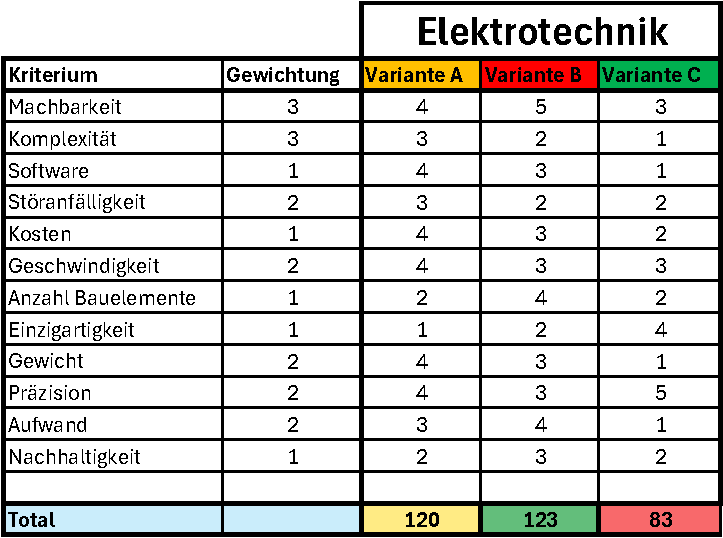
\includegraphics[width=0.75\textwidth]{assets/Nutzwertanalyse-ET.pdf}
\caption{Nutzwertanalyse: Steuerung}
\label{table:nutzwert-ET}
\end{table}

Aus den Bewertungen aus der Nutzwertanalyse zeigt sich die Variante A als höchst bewertete. Somit wird diese Variante weiter verfolgt und besteht aus folgenden Komponenten.

\begin{itemize}
    \item Rechner: Tiny K22
    \item Objekterkennung: Ultraschall
    \item Motoren: Bürstenbehafteter Motor
    \item Anzeige: LEDs 
    \item Akkustische Signalisierung: Lautsprecher
    \item Motorenansteuerung: Treiber einkaufen
    \item Stromversorgung: Akku
    \item Linienerkennung: Fototransistor
    \item Not-Stop: Taster
    \item Inputoption: Schalter
\end{itemize}

\subsubsection{Navigation Nutzwertanalyse}

Die drei ermittelten Varianten aus dem vorherigen Kapitel werden analysiert und bewertet mithilfe einer Nutzwertanalyse.

\begin{itemize}
     \item Variante A - Gelb: Python verwendet eine Mischung aus PyTorch und OpenCV, um AI und reine Bilderkennung zu verwenden. Durch die verschiedenen Moeglichkeiten ist die Entwicklung sehr flexibel. Dijkstra berechnet den Weg. Das Ganze rechnet auf einem Raspberry Pi mit einer Raspberry Camera angeschlossen. Diese Methode ist robust, da zwei Moeglichkeiten zur Erkennung des Graphes verwednet werde nkoennen. Die Kamera und das Board passen gut zusammen und sind recht guenstig. 
    \item  Variante B - Rot: Python verwendet LiteRT, um mit AI die Umgebung zu erkennen und Dijkstra, um den Weg zu berechnen. Das Ganze rechnet auf einem Coral Dev Board und fotografiert den Graphen mit einer Industriekamera. Mit Tensorflow koennte sicher alles erkannt werden, was diese Variante sehr sicher macht. Jedoch ist dies auch ein relativ grosser Algorithmus. Das Coral Dev Board ist staerker als ein Raspberry Pi aber auch teurer.
    \item Variante C - Grün: Python verwendet nur OpenCV zur Bilderkennung und berechnet mit Dijkstra den Weg, es rechnet auf einem Raspberry Pi mit einer Raspberry Camera. Diese Variante koennte schwierig werden, da moeglicherweise nicht alle Elemente erkannt werden koennen, wäre aber sehr leichtgewichtig, da keine AI verwendet wird.
\end{itemize}


\begin{table}[H]
\centering
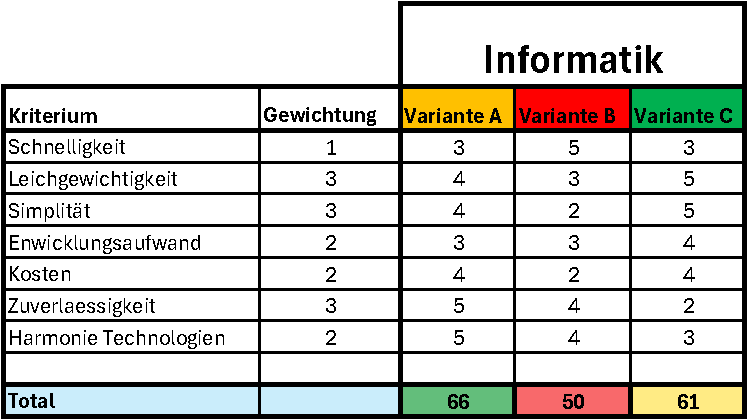
\includegraphics[width=0.75\textwidth]{assets/Nutzwertanalyse-I.pdf}
\caption{Nutzwertanalyse: Navigation}
\label{table:nutzwert-informatik}
\end{table}

Aus der Nutzwertanalyse kann abgelesen werden, dass die Variante A mit Python, PyTorch und OpenCV am besten passt. Die entsprechenden Komponenten aus dieser Variante sind nachfolgend aufgelistet.

\begin{itemize}
    \item Programmiersprache: Python
    \item Bilderkennung: PyTorch und OpenCV
    \item Pathfinding Algorithmus: Dijkstra
    \item Rechner SW: Raspberry Pi
    \item Kamera: Raspberry Camera Modul
\end{itemize}

\subsubsection{Simulator Nutzwertanalyse}

Die drei Varianten wie der Simulator umgesetzt werden könnte, werden bewertet in folgender Nutzwertanalyse. Die Kriterien und deren Gewichtung sind dieselben, wie bei der Nutzwertanalyse für die Informatik im Roboter. Das Ziel des Simulators ist es, diesen möglichst realistisch und wiederverwendbar für \acrshort{pren2} umzusetzen.

\begin{itemize}
    \item Variante A: Ein Java Simulator liest ein JSON File mit dem Basegraph und den Hindernissen und speichert es in einem 2D Array. Durch die Verwendung von Java wäre diese Variante sehr schnell. Bei einem beweglichen Hindernis wird die Gewichtung der Kante erhöht, bei einem Pylonen wird der Knoten entfernt. Dijkstra wird mit einer externen Library implementiert. Die Auswahl des Zielknotens erfolgt zufällig und die Aktivitäten des Roboters werden in einem TUI\footnote{https://en.wikipedia.org/wiki/Text-based\_user\_interface} dargestellt. Im richtigen Roboter wird wahrschienlich nicht Java verwednetet werden. Deswegen koennte der Code hier nicht wiederverwendet werden.
    \item Variante B: Ein Python Simulator liest ein YAML File\footnote{https://yaml.org/} mit dem Basegraph und den Hindernissen und speichert es in einem Dictionary. Dies sind alles leichtgewichtige Technologien. Bei einem beweglichen Hindernis wird die Gewichtung der Kante erhöht, bei einem Pylonen wird der Knoten entfernt. Dijkstra wird selber implementiert, das Ziel kann vom Menschen und zufällig ausgewählt werden und die Aktivitäten des Roboters sind in einem GUI ersichtlich. Der Code kann einfach wiederverwendet werden, unter anderem durch die wenigen externen Abhängigkeiten und die Leichtgewichtigkeit. 
    \item Variante C: Ein Python Simulator liest ein Bild eines Graphens ein und speichert es in einem Graph Datentyp. Bei einem beweglichen Hindernis wird die Gewichtung der Kante erhöht, bei einem Pylonen wird der Knoten entfernt. Eine externe Library implementiert Dijkstra, die Aktivitäten des Roboters werden in einem CLI dargestellt. Es wird bereits an der Bilderkennung gearbeitet, diese müsste folglich bereits früh definiert sein. Dadurch wären bereits viele Aspekte wiederverwendbar.
\end{itemize}

\begin{table}[H]
\centering
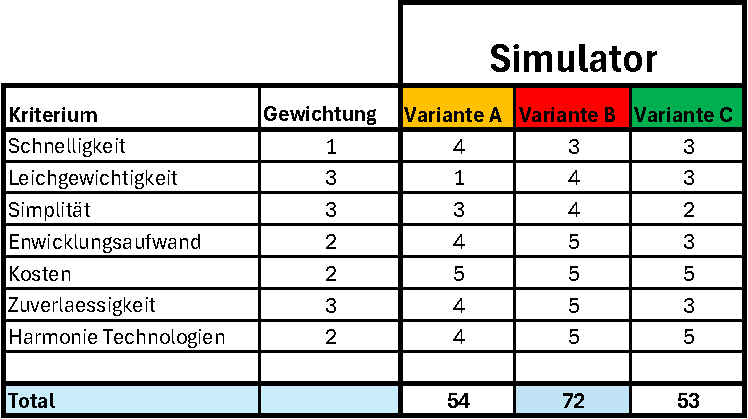
\includegraphics[width=0.75\textwidth]{assets/Nutzwertanalyse-Simulator.pdf}
\caption{Nutzwertanalyse: Simulator}
\label{table:nutzwert-Simulator}
\end{table}

Die Nutzwertanalyse zeigt, dass die Variante B: Python mit YAML und einem GUI am besten abschneidet. Diese Variante besteht aus folgenden Teilen.

\begin{itemize}
    \item Programmiersprache: Python
    \item Wegnetz einlesen: YAML
    \item Wegnetz intern speichern: Key-Values
    \item Bewegliche Hindernisse erfassen: Gewichtung
    \item Blockierte Knoten erfassen: Knoten entfernen
    \item Wegfindung: eigene Implementation
    \item Clientseitige Kommunikation I/O: GUI
\end{itemize}